\documentclass{assignment}
\usepackage{amsmath}
\usepackage{graphicx}
\usepackage{hyperref}
\usepackage{listings}
\usepackage{subfigure}
\usepackage{float}
\usepackage{gensymb}
\usepackage{enumitem}

\coursetitle{Computer Vision I}
\courselabel{CSE 252A}
\exercisesheet{Homework 2}{}
\student{Wei-Yuan Wen, Yen-Ting Chen, Shun-Jen Lee}
\pid{A53202335, A53214417, A53209671}
\university{University of California, San Diego}
\semester{Fall 2016}
\date{November 8, 2016}

\begin{document}
\begin{problemlist}

\pbitem Epipolar Geometry Theory [6 pt]

\textbf{Description:}

Suppose a camera calibration gives a transformation $(R, T)$ such that a point in the world maps to the camera by $^{C}P = R^{W}P + T$.\\

1. Given calibrations of two cameras (a stereo pair) to a common external coordinate system, represented by $R_1, T_1, R_2, T_2$, provide an expression that will map points expressed in the coordinate system of camera 1 to that of camera 2.\\
2. What is the length of the baseline of the stereo pair.\\
3. Give an expression for the Essential Matrix in terms of $R_1, T_1, R_2, T_2$\\

\textbf{Solution:}
1. Assume a point in world coordinate $^WP$, and the mapping equation form world to the cameras are:
\begin{align*}
    ^{C_1}P = R_1^{W}P + T_1\\
    ^{C_2}P = R_2^{W}P + T_2
\end{align*}
And now we map the point from the camera 1 coordinate system to the world one and then the camera 2 one:
\begin{align*}
    &^{W}P = R_1^{T}(^{C_1}P - T_1)\\
    &^{C_2}P = R_2^{W}P + T_2 = R_2R_1^{T}(^{C_1}P-T_1) + T_2
\end{align*}
2.Let $^{C_1}P = O_1$, we have:
\begin{align*}
    ^{C_2}P = -R_2R_1^{T}T_1 + T_2\\
    l = |-R_2R_1^{T}T_1 + T_2|
\end{align*}
3. Assume the origins of two camera $O_1, O_2$ and a point P projected to two image plane $p_1, p_2$, we have:
\begin{align*}
    &p_2(O_2O_1xp_1) = 0\\
    &p_2((-R_2R_1^{T}T_1+T_2)x(R_2R_1^{T}p_1))=0\\
    &\varepsilon = [-R_2R_1^{T}T_1+T_2]_{\times}R_2R_1^{T}
\end{align*}

\newpage
\pbitem Epipolar Geometry [4 pt]

\textbf{Description:}

Consider two cameras whose image planes are the $z$ = 1 plane, and whose focal points are at (−12, 0, 0) and (12, 0, 0). We’ll call a point in the first camera $(x, y)$, and a point in the second camera $(u, v)$. Points in each camera are relative to the camera center. So, for example if $(x, y)$ = (0, 0), this is really the point (−12, 0, 1) in world coordinates, while if $(u, v)$ = (0, 0) this is the point (12, 0, 1).


1. Suppose the points $(x, y)$ = (8, 7) is matched with disparity of 6 to the point $(u, v)$ = (2, 7). What is the 3D location of this point?\\

2. Consider points that lie on the 3-D line $X + Z = 2,Y = 0$. Use the same stereo set up as before. Write an analytic expression giving the disparity of a point on this line after it projects onto the two images, as a function of its position in the right image. So your expression should only involve the variables $u$ and $d$ (for disparity). Your expression only needs to be valid for points on the line that are in front of the cameras, i.e. with $Z > 1$.\\

\textbf{Solution:}

1.We can derive two ray parametric equations from the description in the problem:
\begin{align*}
    x = -12 + 8t, y = 7t, z = t, t\geq1\\
    x = 12 + 2s, y = 7s, z = s, s\geq1
\end{align*}
solving the equations above, we have the intersection of two rays:
\begin{align*}
    t = s = 4
    (x,y,z) = (20,28,4)
\end{align*}
2.Since we know the X and Z of the real point P as $X+Z=2$ and $x_1 = u-d$, we can write down:
\begin{align*}
    X &= \frac{24(u-d)}{-d}\\
    Z &= \frac{24}{-d}\\
    X+Z &= \frac{24u-24d+24}{-d} = 2\\
    d &= \frac{12}{11}u+\frac{12}{11}
\end{align*}

\newpage
\pbitem Reconstruction Accuracy [3pt]

\textbf{Description:}

Characterize the accuracy of the 2D stereo system below. Assume the only source of noise is the localization of corresponding points in the two images (in other words, the only source of error is the disparity). Discuss the dependence of the error in depth estimation $(\Delta Z')$ as a function of baseline width $(b)$, focal length $(f)$, and depth $(Z')$.\\
\textbf{Solution:}\\
As mentioned in lecture 8, we assume that the localization positions of corresponding points in the two images are $X_L$ and $X_R$. By using similar triangles, we have:\\
\begin{center}
$X' = \frac{bX_L}{(X_L-X_R)}, Z' =  \frac{bf}{(X_L-X_R)}$, where $(X_L-X_R)$ is the disparity.\\
\end{center}
To observe the error in depth estimation with respect to the noise of disparity, we differentiate Z' to the disparity. We get:\\
\begin{center}
$\frac{dZ'}{d(X_L-X_R)} = \frac{-bf}{(X_L-X_R)^2}$ $\to$ $\Delta Z' = \frac{-bf}{(X_L-X_R)^2} \Delta(X_L-X_R)$\\
\end{center}
By substituting Z' into the equation, the result becomes:\\
\begin{center}
$\Delta Z' = \frac{-Z'^2}{bf} \Delta(X_L-X_R)$\\
\end{center}
Hence, we can observe that $(\Delta Z')$ is in proportional to the square of estimated depth $(Z'^2)$ and inversely proportional to the product of baseline width $(b)$ and focal length $(f)$.



\newpage
\pbitem Filters as Templates [16pt]

\textbf{Description:}

In this problem we will play with convolution filters. Filters, when convolved with an image, will fire strongest on locations of an image that look like the filter. This allows us to use filters as object templates in order to identify specific objects within an image. In the case of this assignment, we will be finding cars within an image by convolving a car template onto that image. Although this is not a very good way to do object detection, this problem will show you some of the steps necessary to create a good object detector. The goal of this problem will be to teach some pre-processing steps to make vision algorithms be successful and some strengths and weaknesses of filters. Each problem will ask you to analyze and explain your results. If you do not provide an explanation of why or why not something happened, then you will not get full credit. Provide your code in the appendix.\\

\textbf{4.1 Warmup [3pt]}\\
First you will convolve a filter to a synthetic image. The filter or template is \texttt{filter.jpg} and the synthetic image is \texttt{toy.png}. These files are available on the course webpage. You may want to modify the filter image and original slightly. I suggest \texttt{filter\_img = filter\_img - mean(filter\_img(:))}. To convolve the filter image with the toy example, in Matlab you will want to use \texttt{conv2}. The output of the convolution will create an intensity image. Provide this image in the report. In the original image (not the image with its mean subtracted), draw a bounding box of the same size as the filter image around the top 3 intensity value locations in the convolved image. Describe how well you think this technique will work on more realistic images? Do you foresee any problems for this algorithm on more realistic images?\\

\textbf{4.2 Detection Error [3pt]}\\
We have now created an algorithm that produces a bounding box around a detected object. However we have no way to know if the bounding box is good or bad. In the example images shown above, the bounding boxes look reasonable, but not perfect. Given a ground truth bounding box $(g)$ and a predicted bounding box $(p)$, a commonly used measurement for bounding box quality is $\frac{p\cap q}{p\cup q}$. More intuitively, this is the number of overlapping pixels between the bounding boxes divided by the total number of unique pixels of the two bounding boxes combined. Assuming that all bounding boxes will be axis-aligned rectangles, implement this error function and try it on the toy example in the previous section. Choose 3 different ground truth bounding box sizes around one of the Mickey silhouettes. In general, if the overlap is 50\% or more, you may consider that the detection did a good job.\\

\textbf{4.3 More Realistic Images [8pt]}\\
Now that you have created an algorithm for matching templates and a function to determine the quality of the match, it is time to try some more realistic images. The file, \texttt{cartemplate.jpg}, will be the filter to convolve on each of the 5 other car images (\texttt{car1.jpg, car2.jpg, car3.jpg, car4.jpg, car5.jpg}). Each image will have an associated text files that contains 2 $x, y$ coordinates (one pair per line). These coordinates will be the ground truth bounding box for each image. For each car image, provide the following:
\begin{itemize}
    \item A heat map image.
    \item A bounding box drawn on the original image.
    \item The bounding box overlap percent.
    \item A description of what pre-processing steps you needed to do to achieve this overlap.
    \item An explanation of why you felt these steps made sense.
\end{itemize}

\textbf{4.4 Invariance [2pt]}\\
In computer vision there is often a desire for features or algorithms to be invariant to X. One example briefly described in class was illumination invariance. The detection algorithm that was implemented for this problem may have seemed a bit brittle. Can you describe a few things that this algorithm was not invariant to? For example, this algorithm was not scale-invariant, meaning the size of the filter with respect to the size of the object being detected mattered. One filter size should not have worked on everything.\\

\textbf{Solution:}

\textbf{4.1 Warmup:}\\
First, I pre-processed the filter by using \texttt{filter\_img = filter\_img - mean(filter\_img(:))}. Then I used \texttt{conv2} to convolve the filter to the toy image and got an intensity image. The intensity image is shown as Fig.~\ref{fig:4_1subfig:a}.\\
To draw bounding boxes around the top 3 intensity value, I first found the top 3 intensity value and got the responding coordinates. Then I used \texttt{rectangle} to draw bounding boxes of the same size as the filter image around these coordinates in the original image. The result is shown as Fig.~\ref{fig:4_1subfig:b}.\\
I think this technique won't work well on more realistic images since the background of the input image is pretty simple. Also, the filter is pretty as the same size of the object we want to find, so we won't need to do much pre-processing steps on the filter image. If we apply this algorithm on more realistic images, the maximum of the intensity image may not be locate at the object we want to find, since the background will be complicated and distracting. This will mislead us to draw the bounding box on different location in the image. On the other hand, we may not use only a simple filter image to find various kind of object in the same category, or we need to do some more pre-processing steps to get an accurate bounding box.\\

The codes are attached as Listing 1 in Appendix.\\

\textbf{4.2 Detection Error:}\\
I wrote a function named \texttt{detectError}, which takes ground truth box and predicted bounding box as two arguments. Since I have the length and width and at least 2 coordinates of these rectangles, I can easily compute the number of overlapping pixels of the two bounding boxes between the bounding boxes and then divide it by the total number of unique pixels of the two bounding boxes.
I then constructed 3 ground truth bounding boxes having same size as the filter image around one of the Mickey silhouettes and found the overlapping rate are more than 50\%. The result is shown as Fig.~\ref{fig:4_2}.\\

The codes are attached as Listing 3 in Appendix.\\

\newpage
\textbf{4.3 More Realistic Images:}\\
For \texttt{car1} image:
\begin{itemize}
    \item Bounding box overlap percent: 94.72\%.
    \item Pre-processing steps: 
    \begin{enumerate}[label={\alph*)}]
        \item Subtracted both filter image and \texttt{car1} image by their means.
        \item Crop the filter.
        \item Rescale the filter image to the size of ground truth bounding box.
        \item Flip the filter image in x and y dimensions before convolution.
    \end{enumerate}
    \item Explanation: 
    \begin{enumerate}[label={\alph*)}]
        \item I want the object in \texttt{car1} that looks like the filter image has maximums of intensity values, so I subtracted both filter image and \texttt{car1} image by their means.
        \item I cropped the filter image to get rid of the blank area on the top, because I don't want the blank space become a feature.
        \item Then I rescaled the filter image to the size of ground truth bounding box, this way the intensity image will be more accurate and make the maximum locate at the position of \texttt{car1}.
        \item To do the convolution, we need to make sure the filter image is upside down and reversed from left to right, so I flipped it in x and y dimensions right before convolution.
    \end{enumerate}
    \item The result is shown as Fig.~\ref{fig:4_3car1_subfig:a} and Fig.~\ref{fig:4_3car1_subfig:b}.
\end{itemize}

For \texttt{car2} image:
\begin{itemize}
    \item Bounding box overlap percent: 89.59\%.
    \item Pre-processing steps: 
    \begin{enumerate}[label={\alph*)}]
        \item Subtracted both filter image and \texttt{car2} image by their means.
        \item Crop the filter.
        \item Rescale the filter image to the size of ground truth bounding box.
        \item Reverse the filter image from left to right.
        \item Flip the filter image in x and y dimensions before convolution.
    \end{enumerate}
    \item Explanation: 
    \begin{enumerate}[label={\alph*)}]
        \item I want the object in \texttt{car2} that looks like the filter image has maximums of intensity values, so I subtracted both filter image and \texttt{car2} image by their means.
        \item I cropped the filter image to get rid of the blank area on the top, because I don't want the blank space become a feature.
        \item Then I rescaled the filter image to the size of ground truth bounding box, this way the intensity image will be more accurate and make the maximum locate at the position of \texttt{car2}.
        \item I reversed the filter image from left to right, since the head of the car in the \texttt{car2} image points toward right.
        \item To do the convolution, we need to make sure the filter image is upside down and reversed from left to right, so I flipped it in x and y dimensions right before convolution.
    \end{enumerate}
    \item The result is shown as Fig.~\ref{fig:4_3car2_subfig:a} and Fig.~\ref{fig:4_3car2_subfig:b}.
\end{itemize}

For \texttt{car3} image:
\begin{itemize}
    \item Bounding box overlap percent: 50.80\%.
    \item Pre-processing steps: 
    \begin{enumerate}[label={\alph*)}]
        \item Subtracted both filter image and \texttt{car3} image by their means.
        \item Crop the filter.
        \item Rescale the filter image to the size of the rear part of the car in \texttt{car3} image.
        \item Flip the filter image in x and y dimensions before convolution.
    \end{enumerate}
    \item Explanation: 
    \begin{enumerate}[label={\alph*)}]
        \item I want the object in \texttt{car3} that looks like the filter image has maximums of intensity values, so I subtracted both filter image and \texttt{car3} image by their means.
        \item I cropped the filter image to get rid of the blank area on the top, because I don't want the blank space become a feature.
        \item Then I rescaled the filter image to the size of the rear part of the car in \texttt{car3} image, because I thought somehow that rear part looks more alike with the filter image than the side part. This way the intensity image will be more accurate and make the maximum locate at the position of \texttt{car3}.
        \item To do the convolution, we need to make sure the filter image is upside down and reversed from left to right, so I flipped it in x and y dimensions right before convolution.
    \end{enumerate}
    \item The result is shown as Fig.~\ref{fig:4_3car3_subfig:a} and Fig.~\ref{fig:4_3car3_subfig:b}.
\end{itemize}

For \texttt{car4} image:
\begin{itemize}
    \item Bounding box overlap percent: 65.35\%.
    \item Pre-processing steps: 
    \begin{enumerate}[label={\alph*)}]
        \item Subtracted both filter image and \texttt{car2} image by their means.
        \item Crop the filter.
        \item Add 0.1 on each pixel in the filter image.
        \item Rescale the filter image to the size of ground truth bounding box.
        \item Reverse the filter image from left to right.
        \item Flip the filter image in x and y dimensions before convolution.
    \end{enumerate}
    \item Explanation: 
    \begin{enumerate}[label={\alph*)}]
        \item I want the object in \texttt{car4} that looks like the filter image has maximums of intensity values, so I subtracted both filter image and \texttt{car4} image by their means.
        \item I cropped the filter image to get rid of the blank area on the top, because I don't want the blank space become a feature.
        \item I found the top-left area in \texttt{car4} image has similar brightness with the filter image, which  means the intensity is likely to locate at that area. Thus I add 0.1 to every pixels in the filter image to make it brighter.
        \item Then I rescaled the filter image to the size of ground truth bounding box, this way the intensity image will be more accurate and make the maximum locate at the position of \texttt{car4}.
        \item I reversed the filter image from left to right, since the head of the car in the \texttt{car2} image points toward right.
        \item To do the convolution, we need to make sure the filter image is upside down and reversed from left to right, so I flipped it in x and y dimensions right before convolution.
    \end{enumerate}
    \item The result is shown as Fig.~\ref{fig:4_3car4_subfig:a} and Fig.~\ref{fig:4_3car4_subfig:b}.
\end{itemize}

For \texttt{car5} image:
\begin{itemize}
    \item Bounding box overlap percent: 74.40\%.
    \item Pre-processing steps: 
    \begin{enumerate}[label={\alph*)}]
        \item Subtracted both filter image and \texttt{car5} image by their means.
        \item Crop the filter.
        \item Add 0.1 on each pixel in the filter image.
        \item Rescale the filter image to the size of ground truth bounding box.
        \item Reverse the filter image from left to right.
        \item Flip the filter image in x and y dimensions before convolution.
    \end{enumerate}
    \item Explanation: 
    \begin{enumerate}[label={\alph*)}]
        \item I want the object in \texttt{car5} that looks like the filter image has maximums of intensity values, so I subtracted both filter image and \texttt{car5} image by their means.
        \item I cropped the filter image to get rid of the blank area on the top, because I don't want the blank space become a feature.
        \item I found that rhino in \texttt{car5} image and the right part of the forest has similar brightness with the filter image, which means the intensity is likely to locate at that area. Thus I add 0.1 to every pixels in the filter image to make it brighter.
        \item Then I rescaled the filter image to the size of ground truth bounding box, this way the intensity image will be more accurate and make the maximum locate at the position of \texttt{car5}.
        \item I reversed the filter image from left to right, because I thought the trunk of truck in the \texttt{car5} image somehow seems like the head of the filter image.
        \item To do the convolution, we need to make sure the filter image is upside down and reversed from left to right, so I flipped it in x and y dimensions right before convolution.
    \end{enumerate}
    \item The result is shown as Fig.~\ref{fig:4_3car5_subfig:a} and Fig.~\ref{fig:4_3car5_subfig:b}.
\end{itemize}

The codes are attached as Listing 1 to Listing 5 in Appendix.\\

\textbf{4.4 Invariance:}
\begin{enumerate}[label={\alph*)}]
        \item Not color-invariant, the color/brightness of the filter with respect to the color/brightness of the object being detected mattered. We may need to adjust the brightness of the filter to find the correct object in the image. For example, in the \texttt{car4} and \texttt{car5} images, the darker area like smoke, forest and rhinos will mislead us to detect wrong objects.
        \item Not shape-invariant, the silhouette of the filter with respect to the silhouette of the object being detected mattered. For example, in the \texttt{car3} image, we can see that the silhouette of a car may not appear at the correct location we expect.
    \end{enumerate}

\textbf{Result:}

\textbf{4.1 Warmup:}
\begin{figure}[H]
    \begin{center}
        \subfigure[]{
            \label{fig:4_1subfig:a}
            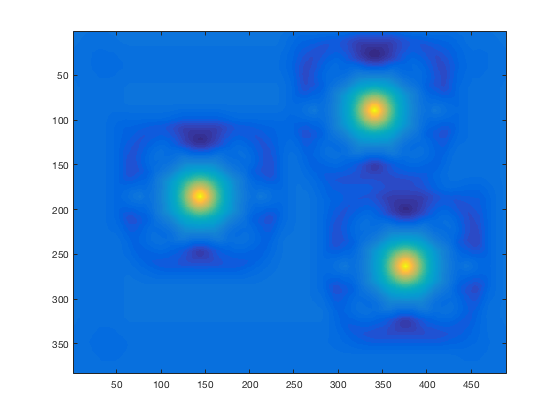
\includegraphics[height = 1.8in]{4_1Intensity_Image}}
        \hspace{0.5cm}
        \subfigure[]{
            \label{fig:4_1subfig:b}
            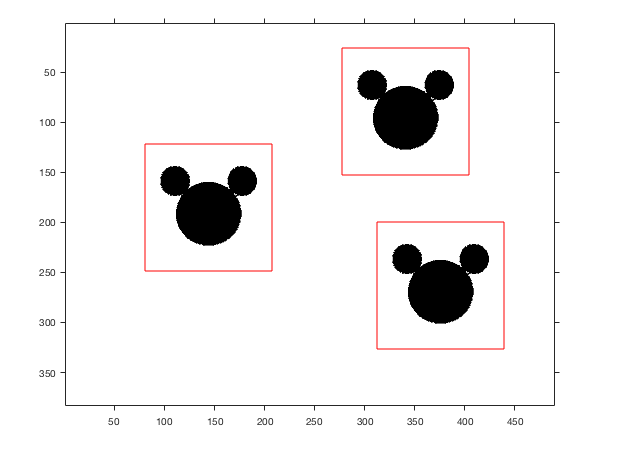
\includegraphics[height = 1.8in]{4_1Bounding_Boxes}}
        \caption{(a) Intensity image, (b) Bounding boxes.}
        \label{fig:4_1images}
    \end{center}
\end{figure}

\textbf{4.2 Detection Error:}
\begin{figure}[H]
\begin{center}
    \includegraphics[height = 2in]{4_2Detection_Error}
    \caption{All overlapping rates of these boxes are greater than 50\%}
    \label{fig:4_2}
\end{center}
\end{figure}

\newpage
\textbf{4.3 More Realistic Images:}
\begin{figure}[H]
    \begin{center}
        \subfigure[]{
            \label{fig:4_3car1_subfig:a}
            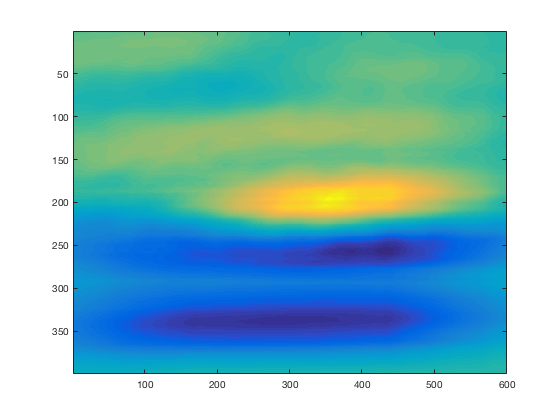
\includegraphics[height = 1.8in]{4_3car1_heat_map}}
        \hspace{0.5cm}
        \subfigure[]{
            \label{fig:4_3car1_subfig:b}
            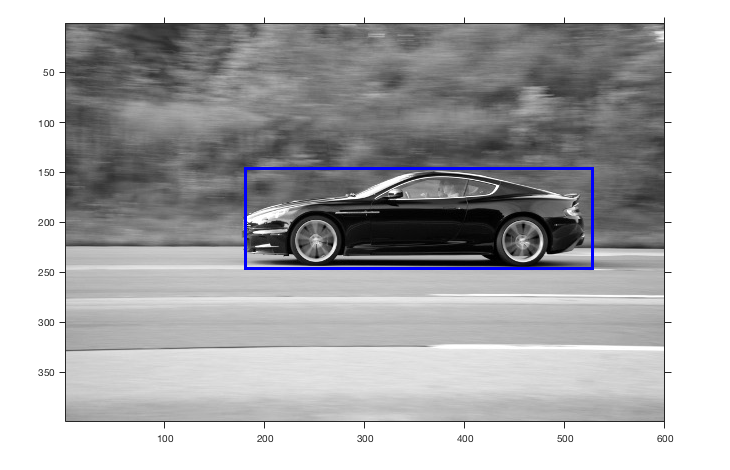
\includegraphics[height = 1.8in]{4_3car1_predicted}}
        \caption{Outputs for \texttt{car1}. (a) Heat map, (b) Bounding boxes.}
        \label{fig:4_3car1_images}
    \end{center}
\end{figure}
\begin{figure}[H]
    \begin{center}
        \subfigure[]{
            \label{fig:4_3car2_subfig:a}
            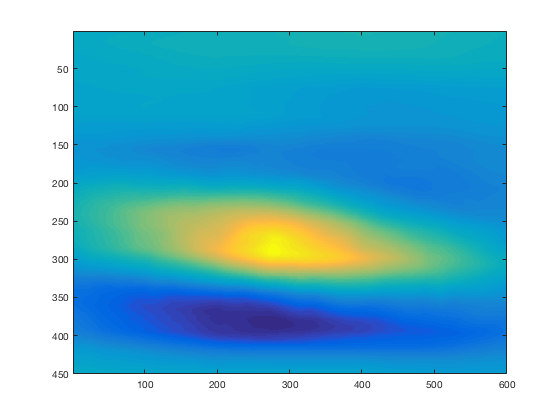
\includegraphics[height = 1.8in]{4_3car2_heat_map}}
        \hspace{0.5cm}
        \subfigure[]{
            \label{fig:4_3car2_subfig:b}
            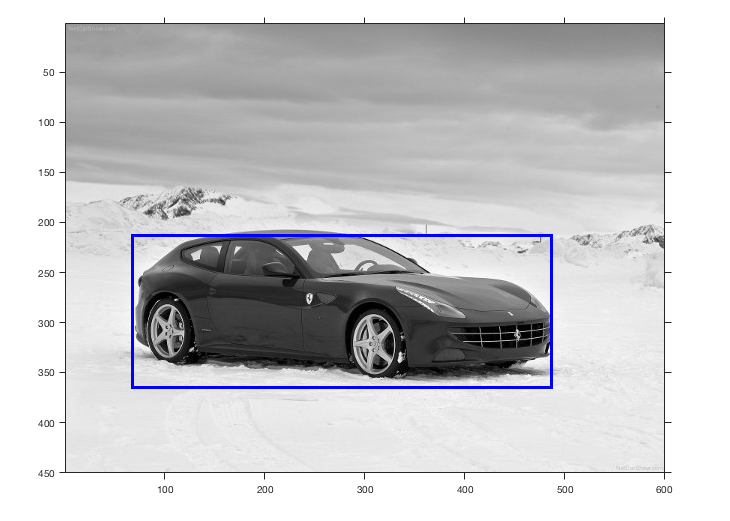
\includegraphics[height = 1.8in]{4_3car2_predicted}}
        \caption{Outputs for \texttt{car2}. (a) Heat map, (b) Bounding boxes.}
        \label{fig:4_3car2_images}
    \end{center}
\end{figure}
\begin{figure}[H]
    \begin{center}
        \subfigure[]{
            \label{fig:4_3car3_subfig:a}
            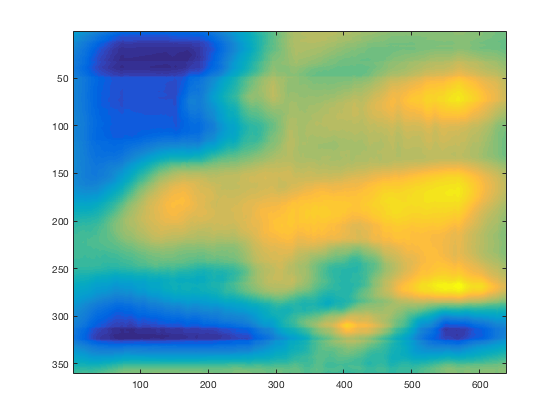
\includegraphics[height = 1.8in]{4_3car3_heat_map}}
        \hspace{0.5cm}
        \subfigure[]{
            \label{fig:4_3car3_subfig:b}
            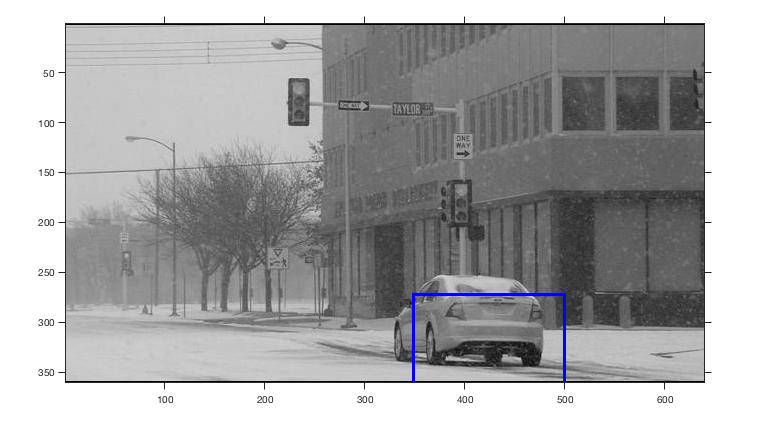
\includegraphics[height = 1.8in]{4_3car3_predicted}}
        \caption{Outputs for \texttt{car3}. (a) Heat map, (b) Bounding boxes.}
        \label{fig:4_3car3_images}
    \end{center}
\end{figure}
\begin{figure}[H]
    \begin{center}
        \subfigure[]{
            \label{fig:4_3car4_subfig:a}
            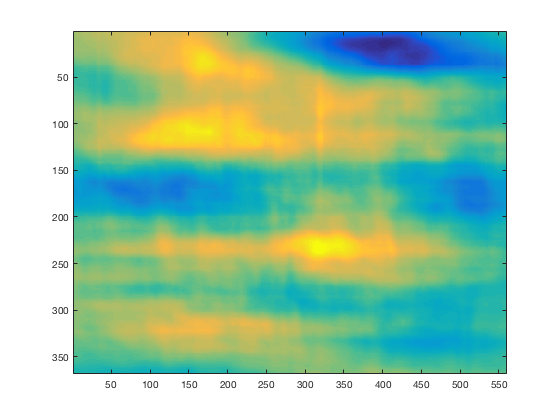
\includegraphics[height = 1.8in]{4_3car4_heat_map}}
        \hspace{0.5cm}
        \subfigure[]{
            \label{fig:4_3car4_subfig:b}
            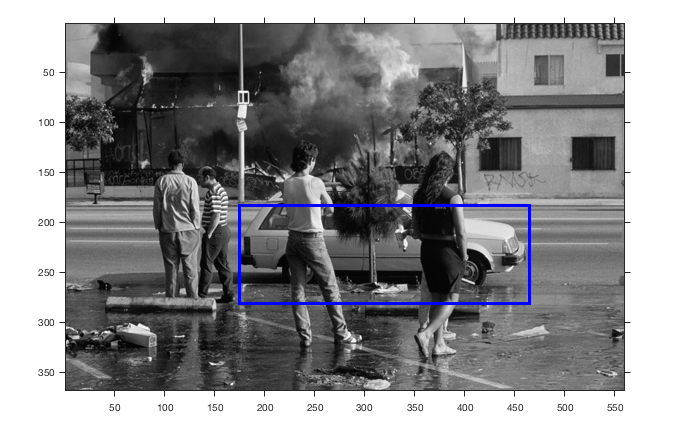
\includegraphics[height = 1.8in]{4_3car4_predicted}}
        \caption{Outputs for \texttt{car4}. (a) Heat map, (b) Bounding boxes.}
        \label{fig:4_3car4_images}
    \end{center}
\end{figure}
\begin{figure}[H]
    \begin{center}
        \subfigure[]{
            \label{fig:4_3car5_subfig:a}
            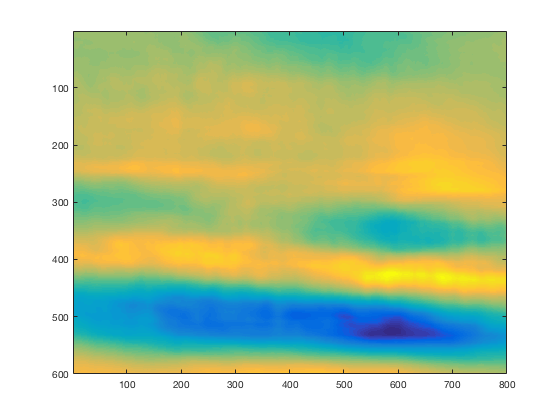
\includegraphics[height = 1.8in]{4_3car5_heat_map}}
        \hspace{0.5cm}
        \subfigure[]{
            \label{fig:4_3car5_subfig:b}
            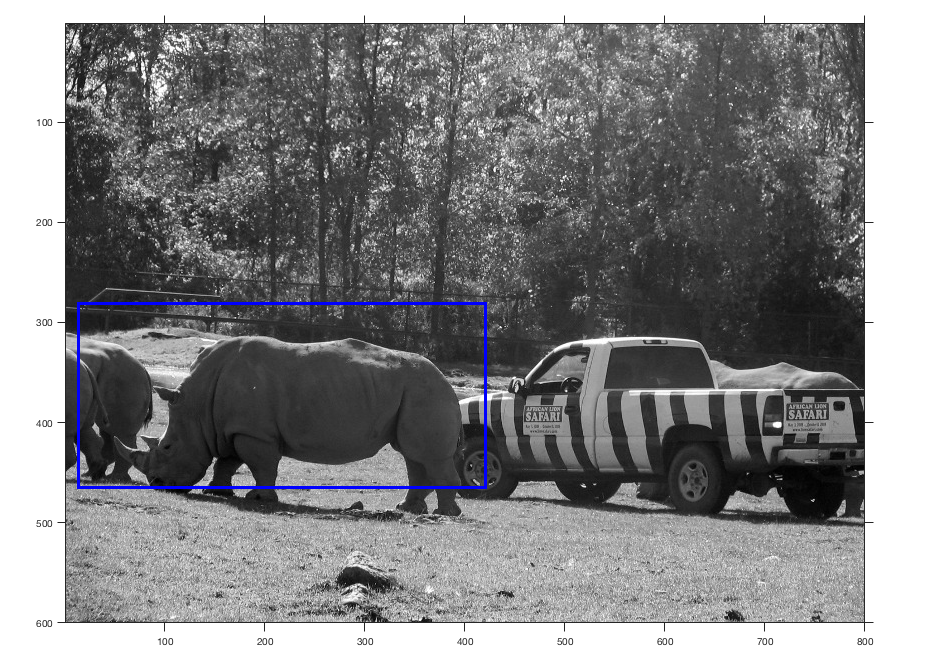
\includegraphics[height = 1.8in]{4_3car5_predicted}}
        \caption{Outputs for \texttt{car5}. (a) Heat map, (b) Bounding boxes.}
        \label{fig:4_3car5_images}
    \end{center}
\end{figure}

\newpage
\pbitem Canny Edge Detection [9pt]

\textbf{Description:}

In this problem, you have to write a function to do CANNY EDGE DETECTION. The following steps need to be implemented.
\begin{itemize}
    \item\textbf{Smoothing [1pt]:} First, we need to smooth the images to remove noise from being considered as edges. For this assignment, use a 5$\times$5 Gaussian kernel filter 1 with σ = 1.4 to smooth the images.\\
    \begin{align}
        K = \frac{1}{159}
        \begin{bmatrix}
        2&4&5&4&2\\
        4&9&12&9&4\\
        5&12&12&12&5\\
        4&9&12&9&4\\
        2&4&5&4&2
        \end{bmatrix}
    \end{align}
    
    \item\textbf{Gradient Computation [2pt]:}
    After you have finished smoothing, find the image gradient in the horizontal and vertical directions. You can use Sobel operators 2 as your filter kernel to calculate $G_x$ and $G_y$. $G_x$ and $G_y$ are the gradients along the $x$ and $y$ axis respectively. $s_x$ and $s_y$ are the corresponding kernels. Compute the gradient magnitude image as $|G| = \sqrt{G^{2}_x + G^{2}_y}$. The edge direction as each pixel is given as $G_{\theta} = \tan^{-1}(\frac{G_x}{G_y}).$
    \begin{align}
        s_x =
        \begin{bmatrix}
        -1&0&1\\
        -2&0&2\\
        -1&0&1\\
        \end{bmatrix},
        s_y =
        \begin{bmatrix}
        -1&-2&-1\\
        0&0&0\\
        1&2&1\\
        \end{bmatrix}.
    \end{align}
    
    \item\textbf{Non Maximum Suppression [3pt]:}
    Our desired edges need to be sharp, not thick like the ones in gradient image. Use non maximum suppression to preserve all local maximas and discard the rest. You can use the following method to do so:\\
    For each pixel do:\\
    $\bullet$ Round the gradient direction $\theta$ to the nearest multiple of 45$\degree$ in a 8-connected neighbourhood.\\
    $\bullet$ Compare the edge strength at the current pixel to the pixels along the $+ve$ and $−ve$ gradient direction in the 8-connected neighbourhood.\\
    $\bullet$ Preserve the values of only those pixels which have maximum gradient magnitudes in the neighbourhood along the $+ve$ and $−ve$ gradient direction.\\
        
    \item\textbf{Hysteresis Thresholding [3pt]:}
    Choose optimum values of thresholds and use the thresh- olding approach given in lecture 7. This will remove the edges caused due to noise and colour variations.
\end{itemize}
Compute the images after each step and select suitable thresholds that retains most of the true edges. For this question use the image \texttt{geisel.jpeg} in the data folder.\\

\newpage
\textbf{Solution:}

For smoothing, I used \texttt{conv2.m} and applied the Gaussian filter with $\sigma$ = 1.4 to smooth the image. The result is shown as Fig.~\ref{fig:5subfig:a}.

For gradient computation, I use $s_x$ and $s_y$ to calculate $G_x$ and $G_y$ respectively. Then I computed the gradient magnitude image using $|G| = \sqrt{G^{2}_x + G^{2}_y}$ and get the edge direction at each pixel by computing $G_{\theta} = \tan^{-1}(\frac{G_x}{G_y}).$ The result is shown as Fig.~\ref{fig:5subfig:b}.

For non maximum suppression, I first rounded every gradient direction at each pixel to the nearest multiple of 45$\degree$. And for each pixel, I checked if the gradient magnitude of two pixels along the $+ve$ and $−ve$ gradient direction in the 8-connected neighbourhood is smaller than that of current pixel. If both magnitudes are smaller, I added the current pixel to the edge candidate. The result is shown as Fig.~\ref{fig:5subfig:c}.

For hysteresis thresholding, I set $\tau_{high} = 0.4$ and $\tau_{low} = 0.1$, I first added all the pixels, which have values higher than $\tau_{high}$, from edge candidate into an dynamic array. For each pixel in the array, I added it into a result map and added pixels within 8-connected neighbourhood of it into the array if those pixels' gradient magnitude are higher than $\tau_{low}$ and are not already in the result map. The result is shown as Fig.~\ref{fig:5subfig:d}.

The codes are attached as Listing 6 to Listing 7 in Appendix.\\

\textbf{Result:}

\begin{figure}[H]
\begin{center}
    \includegraphics[height = 1.8in]{5_0Geisel}
    \caption{Original Image}
    \label{fig:5geisel}
\end{center}
\end{figure}

\begin{figure}[H]
    \begin{center}
        \subfigure[]{
            \label{fig:5subfig:a}
            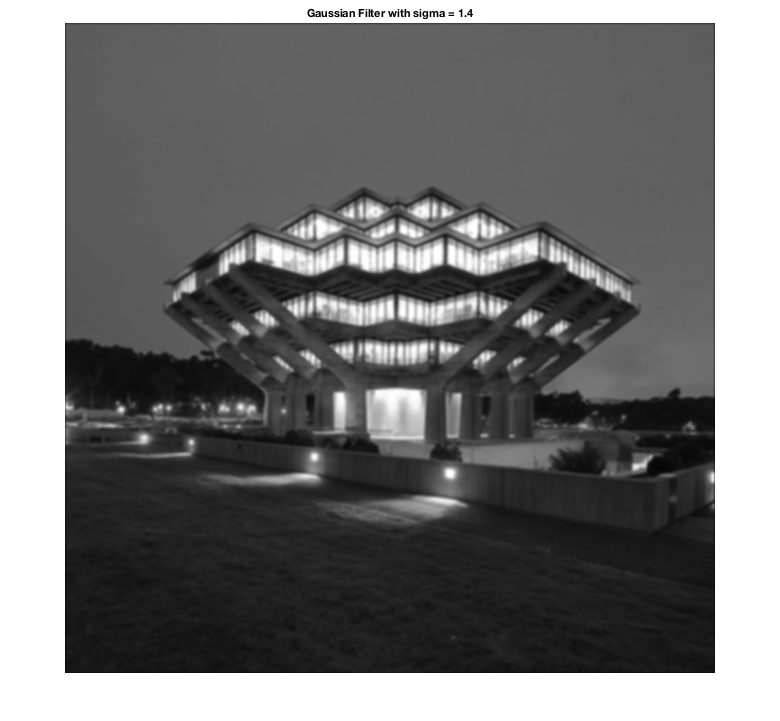
\includegraphics[height = 1.8in]{5_1Gaussian}}
        \hspace{0.5in}
        \subfigure[]{
            \label{fig:5subfig:b}
            \includegraphics[height = 1.8in]{5_2Gradient_Magnitude}}
        \label{fig:images}
        \vspace{0.5cm}
        \subfigure[]{
            \label{fig:5subfig:c}
            \includegraphics[height = 1.8in]{5_3Non_Maximum_Suppression}}
        \hspace{0.5in}
        \subfigure[]{
            \label{fig:5subfig:d}
            \includegraphics[height = 1.8in]{5_4Hysteresis_Thresholding}}
        \caption{(a) Smoothed Image using Gaussian filter with $\sigma = 1.4$, (b) Gradient Magnitude, (c) Non Maximum Suppression edges, (d) Final Edge after Hysteresis Thresholding.}
        \label{fig:5images}
    \end{center}
\end{figure}

\newpage
\pbitem Sparse Stereo Matching [27pt]

\textbf{Description:}

In this problem we will play around with sparse stereo matching methods. You will work on two image pairs, a warrior figure and a figure from the Matrix movies (\texttt{warrior2.mat} and \texttt{matrix2.mat}). These files both contain two images, two camera matrices, and set sets of corresponding points (extracted by manually clicking the images). For illustration, I have run my code on a third image pair (\texttt{dino2.mat}). This data is also provided on the webpage for you to debug your code, but you should only report results on warrior and matrix. In other words, where I include one (or a pair) of images in the assignment below, you will provide the same thing but for BOTH matrix and warrior. Note that the matrix image pair is harder, in the sense that the matching algorithms we are implementing will not work quite as well. You should expect good results, however, on warrior. To make the TAs extra happy, make the line width and marker sizes bigger than the default sizes.\\

\textbf{6.1 Corner Detection [8pt]}\\
The first thing we need to do is to build a corner detector. This should be done according to \texttt{http://cseweb.ucsd.edu/classes/fa16/cse252A-a/lec7.pdf}. Your file should be named\\
\texttt{CornerDetect.m}, and take as input\\
\begin{lstlisting}
corners = CornerDetect(Image, nCorners, smoothSTD, windowSize)
\end{lstlisting}
where \texttt{smoothSTD} is the standard deviation of the smoothing kernel, and \texttt{windowSize} the size of the smoothing window. In the lecture the corner detector was implemented using a hard threshold. Do not do that but instead return the \texttt{nCorners} strongest corners after non-maximum suppression. This way you can control exactly how many corners are returned. Run your code on all four images (with \texttt{nCorners} = 20) and show outputs.\\
\textbf{Solution:}\\
To detect the corners, we follow the method in lecture 7.\\
1. Filter image with a Gaussian.\\
2. Compute the gradient in both x and y directions for every pixel.\\
3. Move window over image, and for each window location: \\
(1) Construct the matrix C over the window.\\
\begin{center}
$
C(x, y) =
\left(
\begin{array}{clr}
\sum{}I_x^2 & \sum{}I_xI_y\\
\sum{}I_xI_y & \sum{}I_y^2
\end{array}
\right)
$
\end{center}
(2) Find the eigenvalue for C using eig() in matlab.\\
(3) Store the smaller eigenvalue for every pixel in a matrix.\\
4. Perform non-maximum suppression by comparing the stored eigenvalue in every pixel with its neighbors(a window). If the eigenvalue is the maximum in the window, we take this pixel as a candidate of a corner.\\
5. We sort all the candidates by their eigenvalues, and choose the largest nCorners pixels as our result.\\
\newpage
\textbf{Result:}

\begin{figure}[!ht]
\centering
\subfigure{
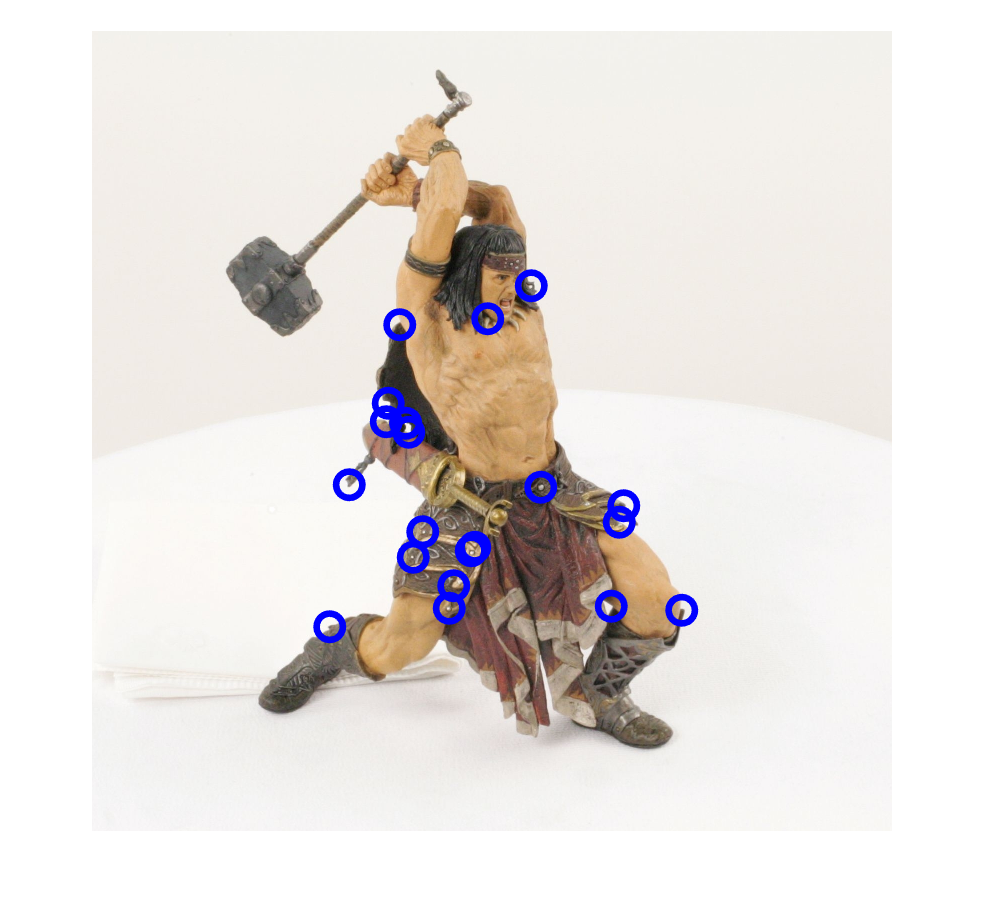
\includegraphics[height = 2.8 in]{6_1warrior1.png}}
\subfigure{
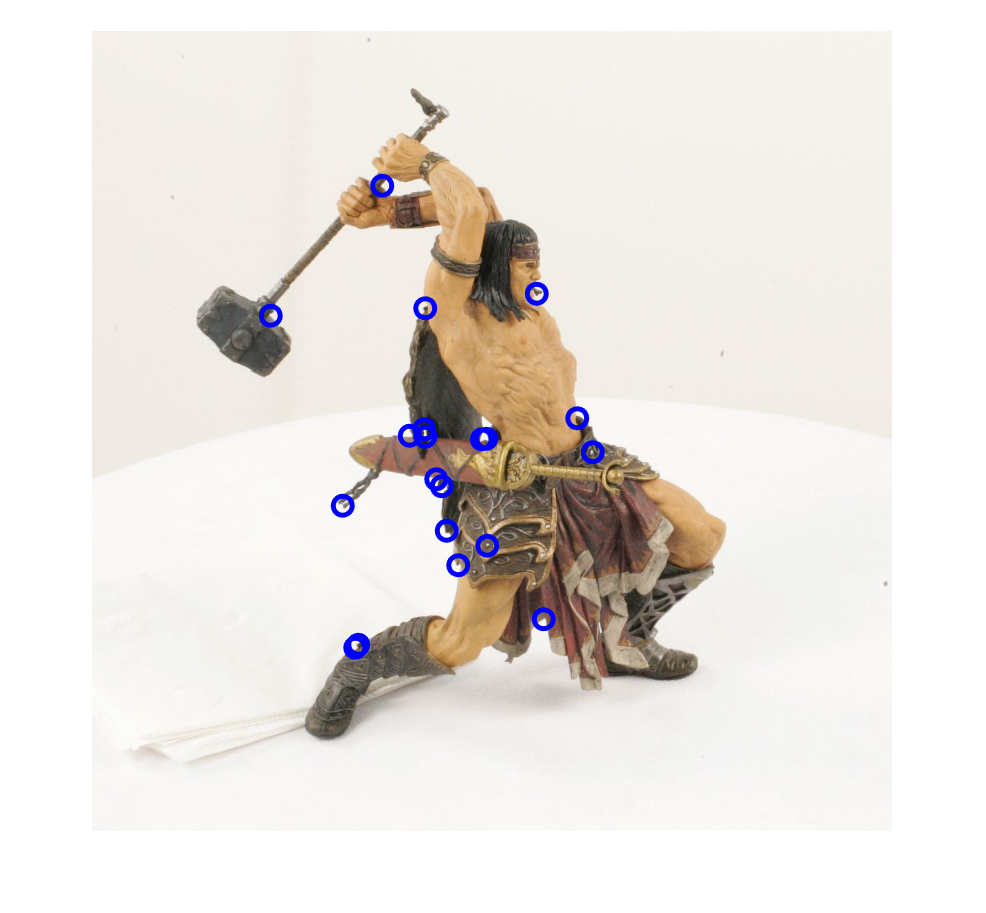
\includegraphics[height = 2.8 in]{6_1warrior2.png}}
\caption{Corner Detection: Warrior}
\end{figure}

\begin{figure}[!ht]
\centering
\subfigure{
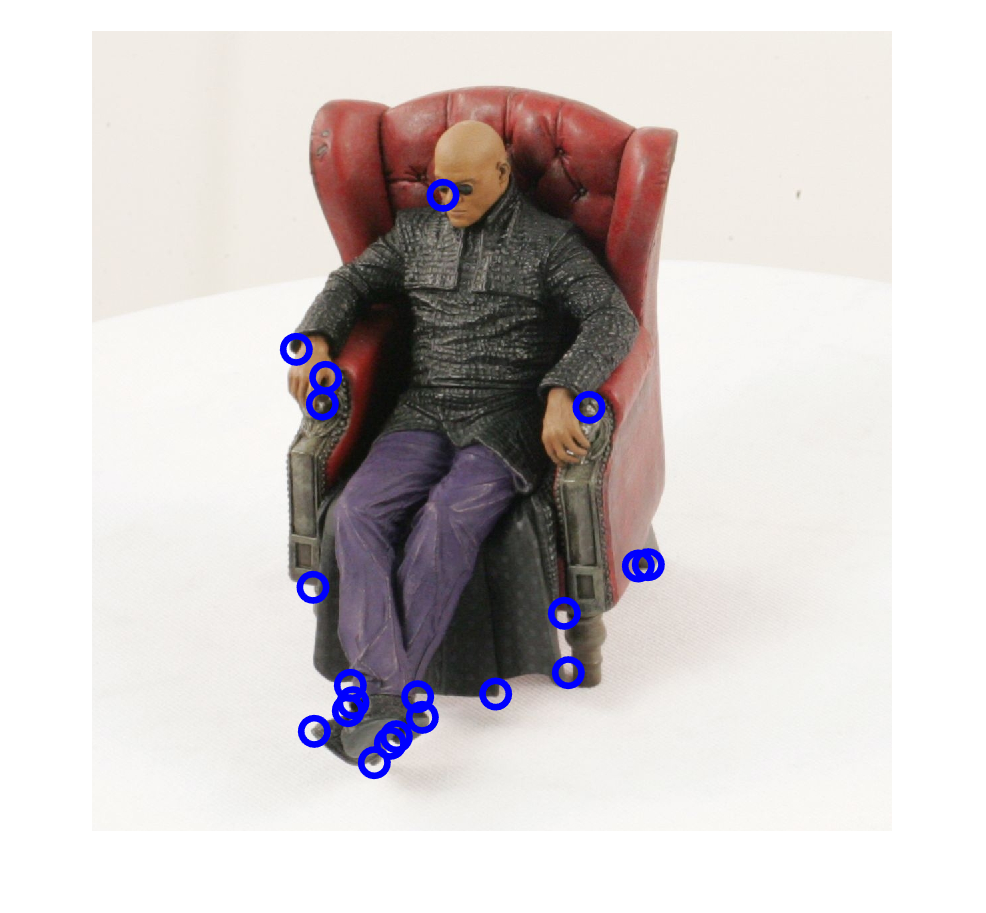
\includegraphics[height = 2.8 in]{6_1matrix1.png}}
\subfigure{
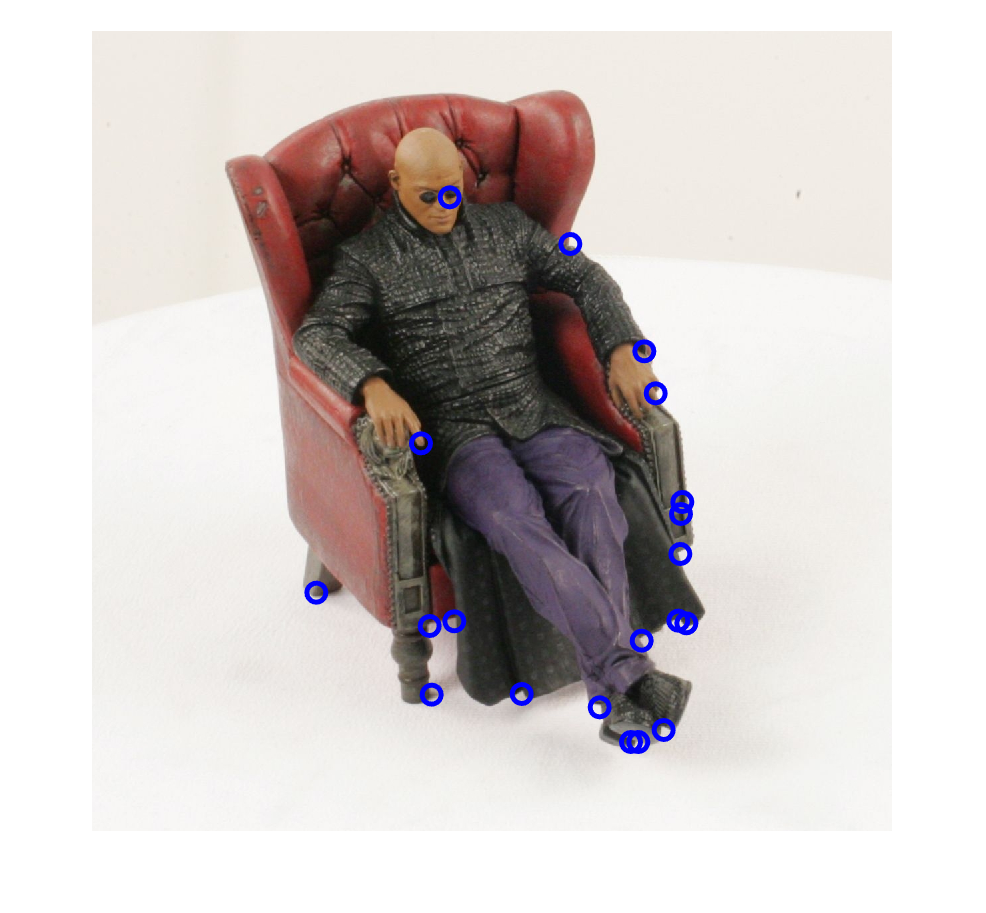
\includegraphics[height = 2.8 in]{6_1matrix2.png}}
\caption{Corner Detection: Matrix}
\end{figure}

\newpage
\textbf{6.2 SSD Matching [2pt]}\\
Write a function \texttt{SSDmatch.m} that implements the SSD matching algorithm for two input windows. Include this code in your report (in appendix as usual).\\
\textbf{Solution:}\\
To implement the SSD matching algorithm, we simply vectorizes the two input windows and then take the 2-norm of their difference.\\

\textbf{6.3 Naive Matching [4pt]}\\
Equipped with the corner detector and the SSD matching code, we are ready to start finding correspondances. One naive strategy is to try and find the best match between the two sets of corner points. Write a script that does this, namely, for each corner in image1, find the best match from the detected corners in image2 (or, if the SSD match score is too low, then return no match for that point). You will have to figure out a good threshold (SSDth) value by experimentation. Write a function \texttt{naiveCorrespondanceMatching.m} and call it as below. Examine your results for 10, 20, and 30 detected corners in each image. In your report, only include your results for 10 corners, so that the figure will not be cluttered. \texttt{naiveCorrespondanceMatching.m} will call your SSD mathch- ing code. The parameter \texttt{R} below, is the radius of the patch used for matching.\\
\begin{lstlisting}
ncorners = 10;
corners1 = CornerDetect(I1, ncorners, smoothSTD, windowSize));
corners2 = CornerDetect(I2, ncorners, smoothSTD, windowSize));
[I, corsSSD] = naiveCorrespondanceMatching(I1, I2, corners1, corners2, R, SSDth);
\end{lstlisting}
\textbf{Solution:}\\
We simply follow the instruction above to search the best match in image2 for every corner in image1. We adjust the SSD threshold so that it can have the highest percentage of correct matches. In the end, we got 4 correct matches among 7 matches in Warrior images and 3 correct matches among 9 matches in Matrix images.\\
\newpage
\textbf{Result:}
\begin{figure}[!ht]
\centering
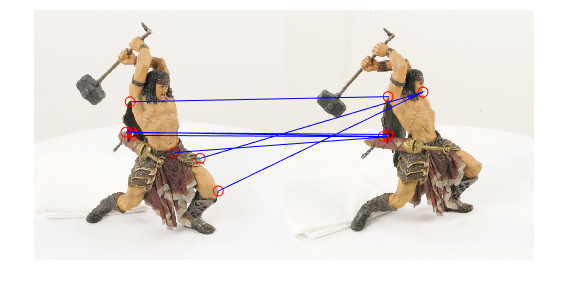
\includegraphics[scale = 1.0]{6_3warrior.png}
\caption{Naive Matching: Warrior}
\end{figure}

\begin{figure}[!ht]
\centering
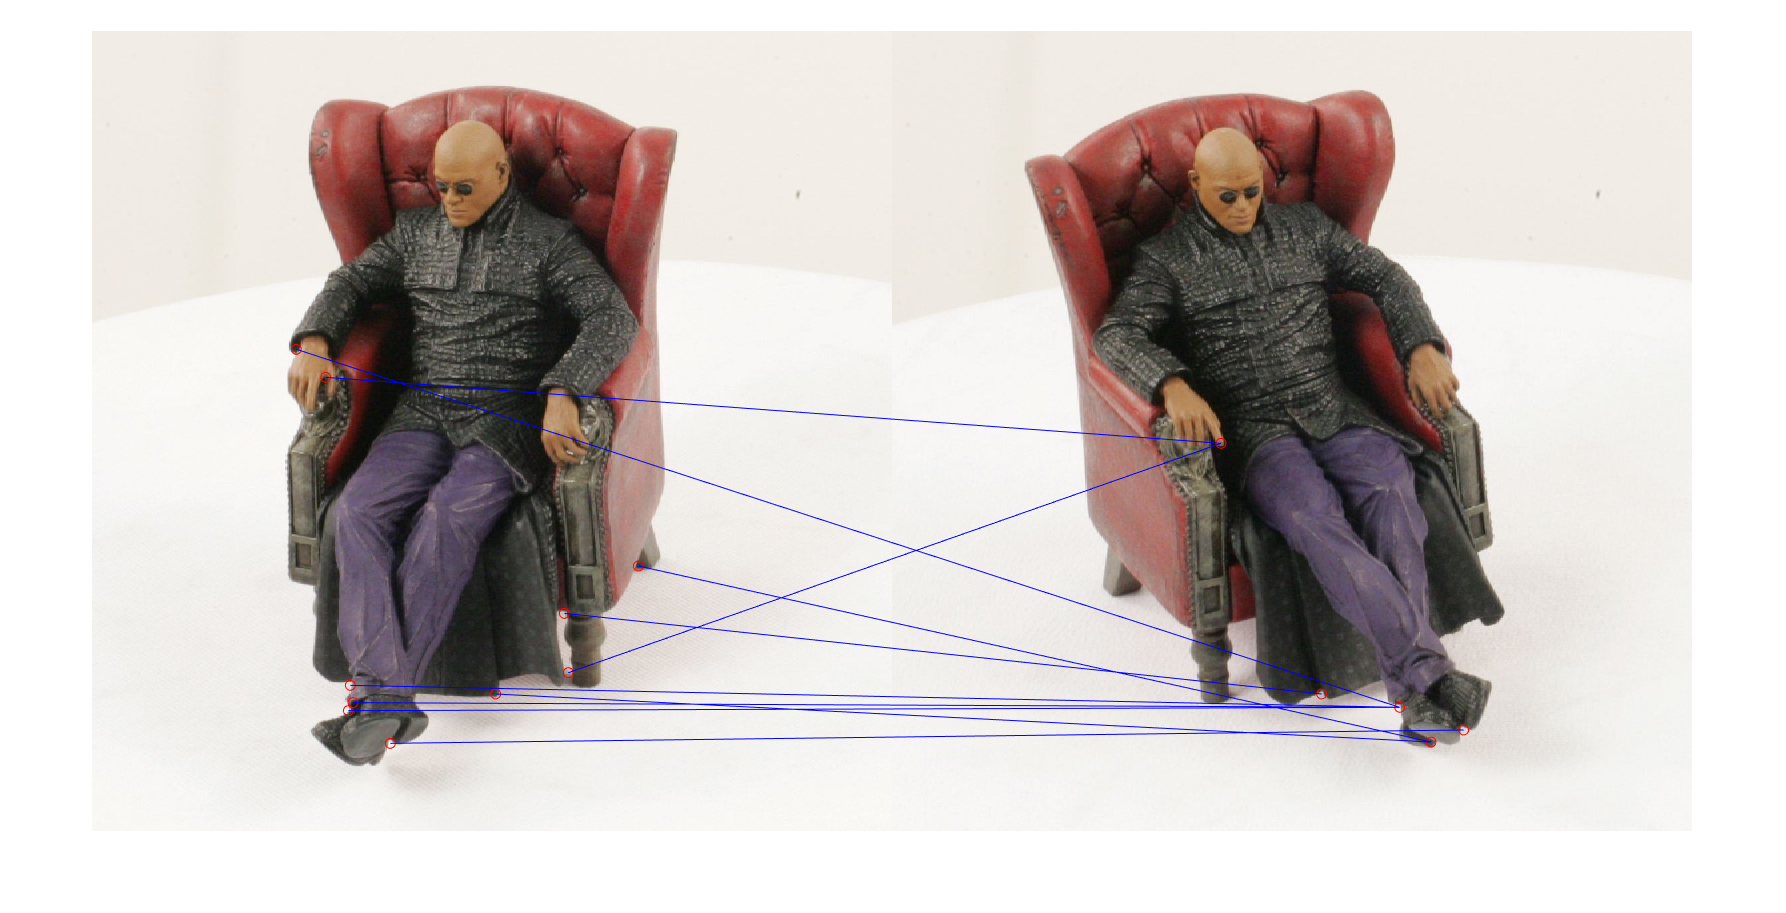
\includegraphics[scale = 1.0]{6_3matrix.png}
\caption{Naive Matching: Matrix}
\end{figure}

\newpage
\textbf{6.4 Epipolar Geometry [3pt]}\\
Using the provided \texttt{fund.m} together with the provided points \texttt{cor1}, and \texttt{cor2}, calculate the fundamental matrix, and then plot the epipolar lines in both images pairs as shown below. Plot the points and make sure the epipolar lines go through them. You might find the supplied \texttt{linePts.m} function useful when you are working with epipolar lines.\\
\textbf{Solution:}\\
To compute the epipolar line in image1 for the the corner in image2, we use $l_1 = \textbf{F}^Tp_2$\\
To compute the epipolar line in image2 for the the corner in image1, we use $l_2 = \textbf{F}p_1$\\
The \textbf{F} above is the fundimental matrix.\\
\textbf{Result:}
\begin{figure}[!ht]
\centering
\subfigure{
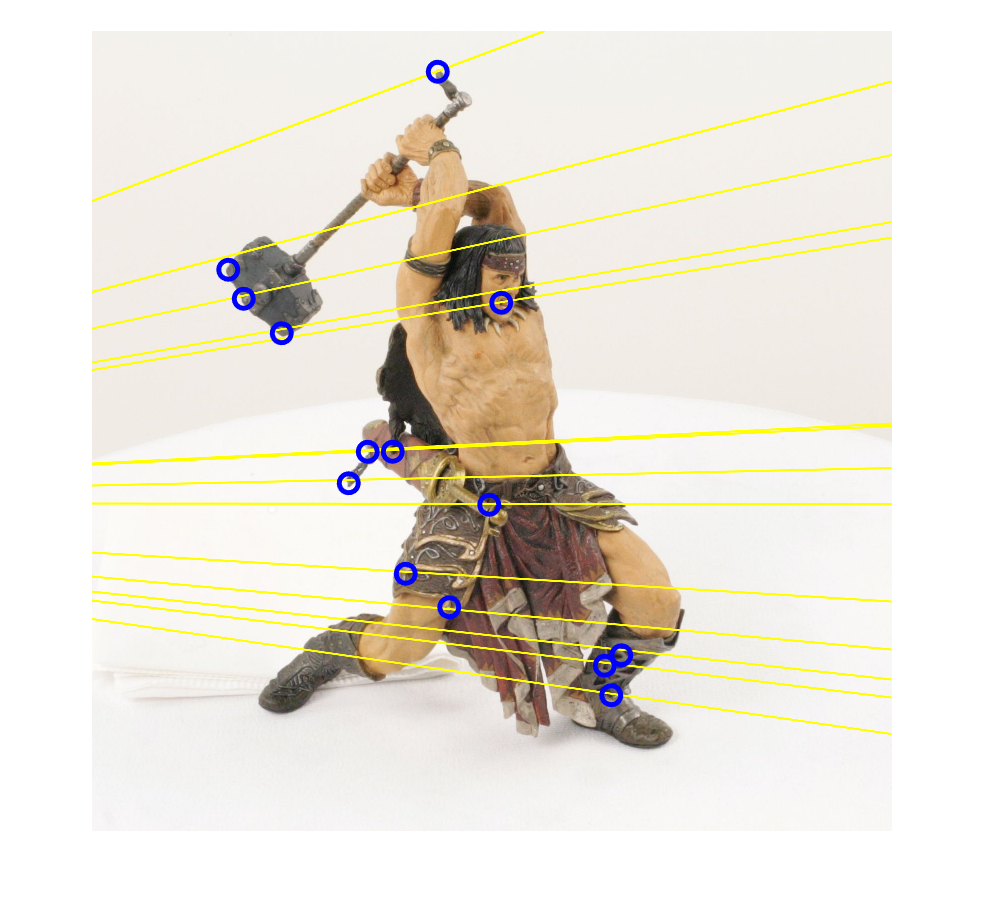
\includegraphics[height = 2.3 in]{6_4warrior1.png}}
\subfigure{
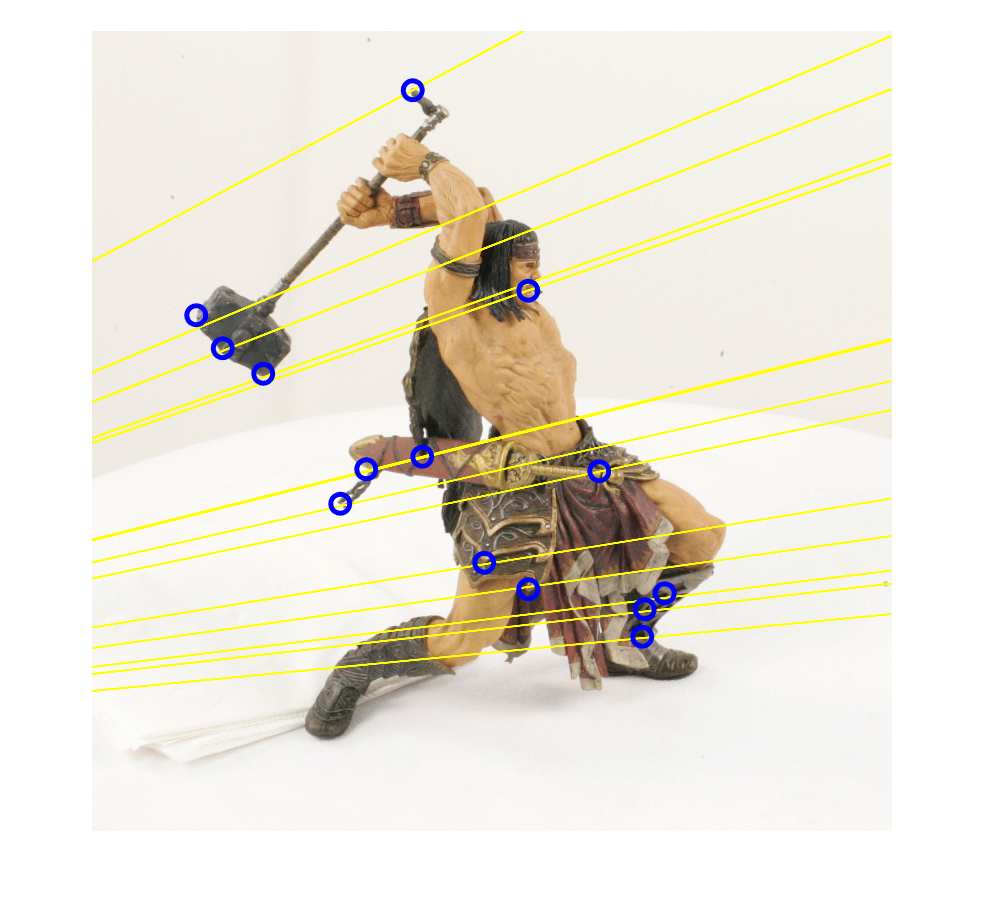
\includegraphics[height = 2.3 in]{6_4warrior2.png}}
\caption{Epipolar Lines: Warrior}
\end{figure}

\begin{figure}[!ht]
\centering
\subfigure{
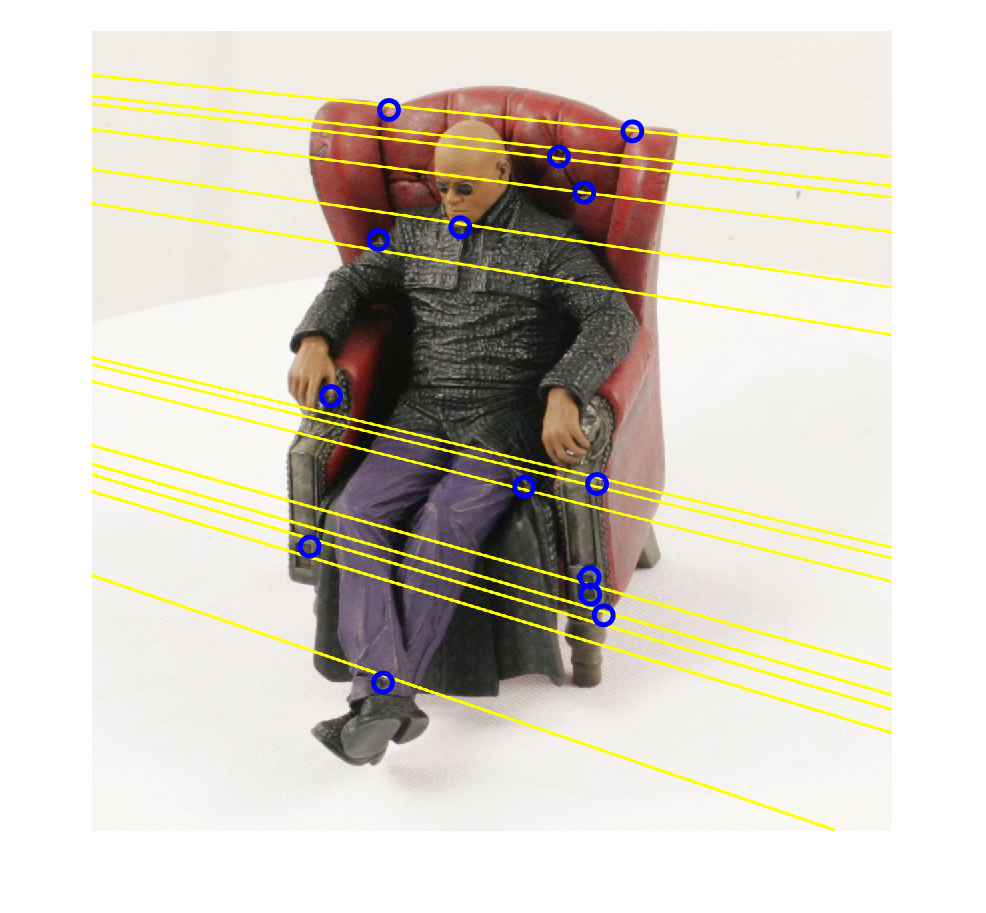
\includegraphics[height = 2.3 in]{6_4matrix1.png}}
\subfigure{
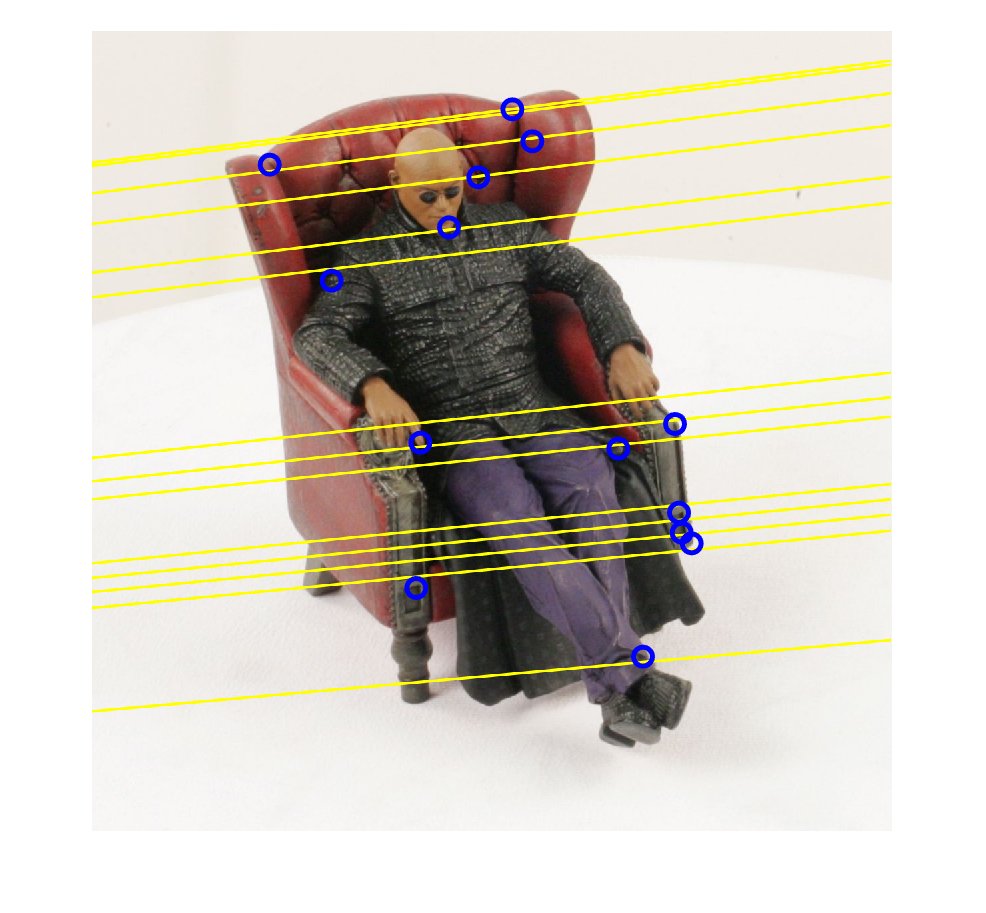
\includegraphics[height = 2.3 in]{6_4matrix2.png}}
\caption{Epipolar Lines: Matrix}
\end{figure}


\newpage
\textbf{6.5 Epipolar Geometry Based Matching [5pt]}\\
We will now use the epipolar geometry to build a better matching algorithm. First, detect 10 corners in Image1. Then, for each corner, do a linesearch along the corresponding epipolar line in Image2. Evaluate the SSD score for each point along this line and return the best match (or no match if all scores are below the SSDth). \texttt{R} is the radius (size) of the SSD patch in the code below. You do not have to run this in both directions, but only as indicated in the code below.\\
\begin{lstlisting}
ncorners = 10;
F = fund(cor1, cor2);
corners1 = CornerDetect(I1, ncorners, smoothSTD, windowSize));
corsSSD = correspondanceMatchingLine( I1, I2, corners1, F, R, SSDth);
\end{lstlisting}
\textbf{Solution:}\\
To do the linesearch, we have to interpolate the pixels from the line. We interpolate the pixels by first using the supplied \texttt{linePts.m} to find the two end points of the line. Then for every x and y in between these end points, we compute a corresponding y and x by the slope of the line.\\
The other processes are as same as the processes in 6.3.\\
\newpage
\textbf{Result:}
\begin{figure}[!ht]
\centering
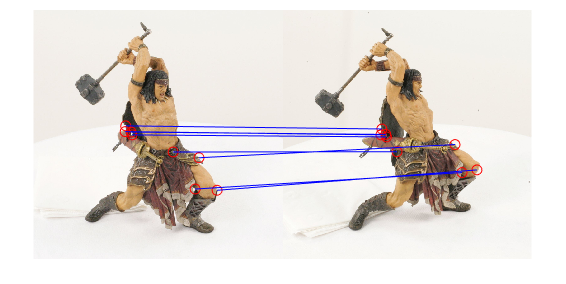
\includegraphics[scale = 1.0]{6_5warrior.png}
\caption{Epipolar Geometry Based Matching: Warrior}
\end{figure}

\begin{figure}[!ht]
\centering
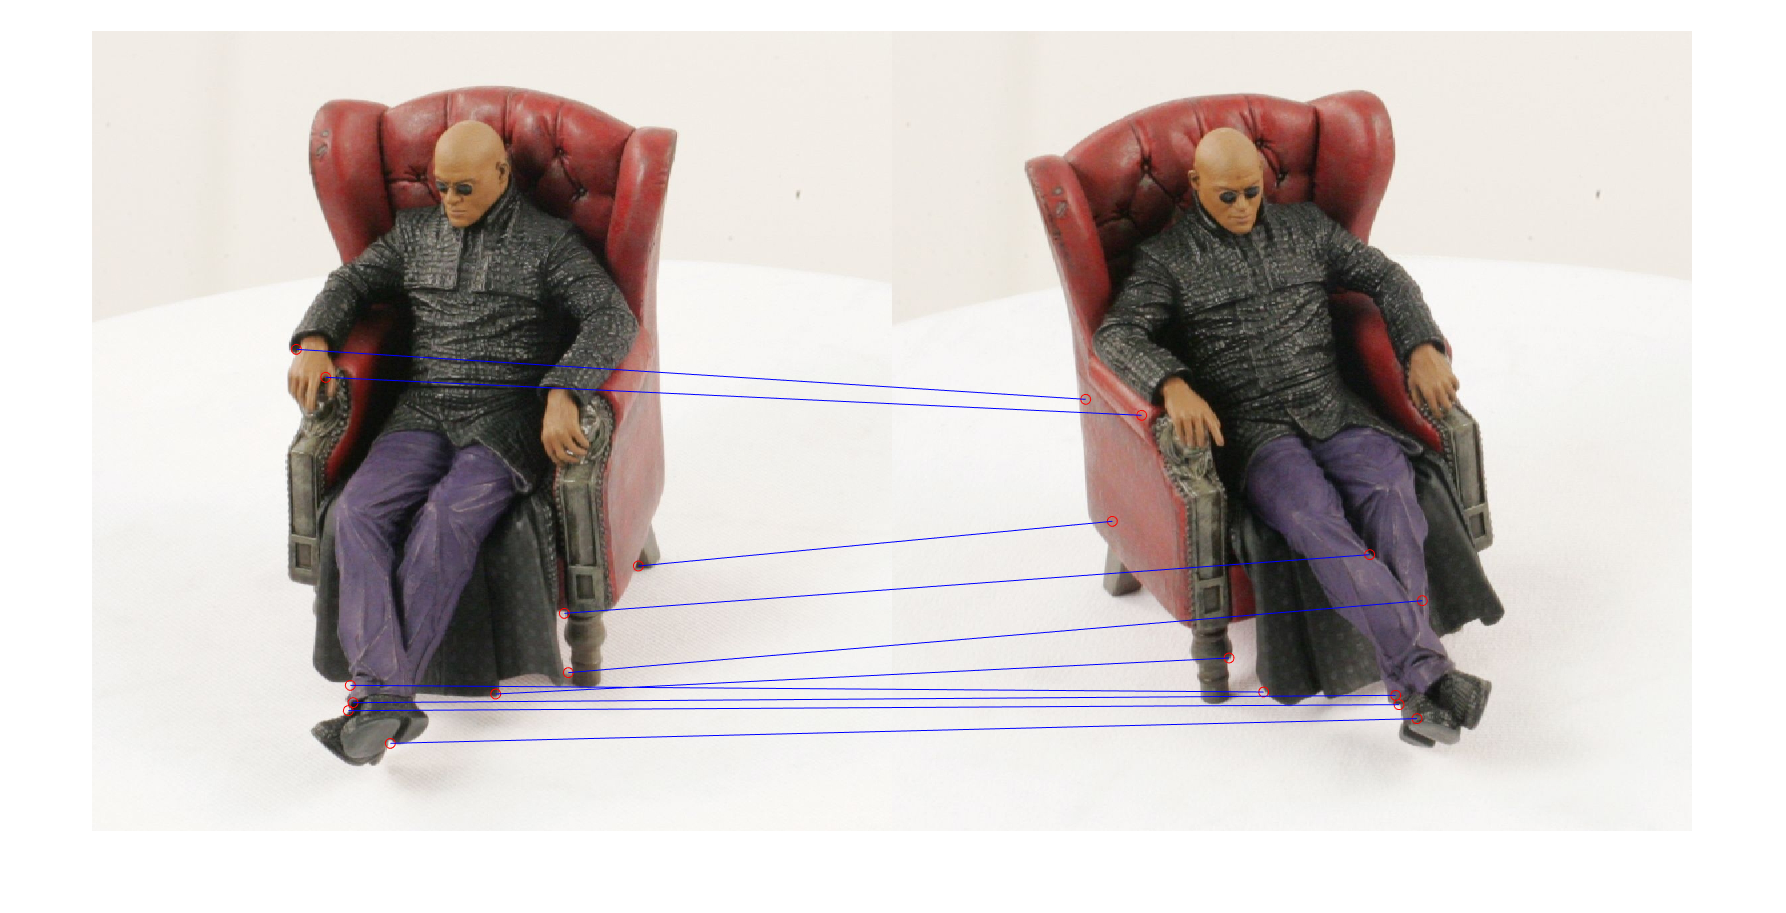
\includegraphics[scale = 1.0]{6_5matrix.png}
\caption{Epipolar Geometry Based Matching: Matrix}
\end{figure} 

\newpage
\textbf{6.6 Triangulation [5pt]}\\
Now that you have found correspondences between the pairs of images we can triangulate the corresponding 3D points. Since we do not enforce the ordering constraint the correspondences you have found are likely to be noisy and to contain a fair amount of outliers. Using the provided camera matrices you will triangulate a 3D point for each corresponding pair of points. Then by reprojecting the 3D points you will be able to find most of the outliers. You should implement the linear triangulation method described in lecture. \texttt{P1} and \texttt{P2} below are the camera matrices. Also write a function, \texttt{findOutliers.m}, that reprojects the world points to Image2, and then determines which points are outliers and inliers respectively. For this purpose, we will call a point an outlier if the distance between the true location, and the reprojected point location is more than 20 pixels.\\
\begin{lstlisting}
outlierTH = 20;
F = fund(cor1, cor2);
ncorners = 50;
corners1 = CornerDetect(I1, ncorners, smoothSTD, windowSize));
corsSSD = correspondanceMatchingLine( I1, I2, corners1, F, R, SSDth);
points3D = triangulate(corsSSD, P1, P2);
[ inlier, outlier ] = findOutliers(points3D, P2, outlierTH, corsSSD);
\end{lstlisting}
Display your results by showing, for Image2, the original points in black circles, the inliers as blue plus signs, and the outliers as red plus signs, as shown in Figure 7. Compare this outlierplot with Figure 6. Does the detected outliers correspond to false matches?

\textbf{Solution:}
To implement the triangulation, we use the linear triangulation method described in lecture. First, for a pair of corresponding corners in image1 and image2, we each construct two lines that passes the corner. We choose the lines simply by
\begin{center}
$x + y - (x_1 + y_1) = 0$\\
$x - y - (x_1 - y_1) = 0$\\
$x + y - (x_2 + y_2) = 0$\\
$x - y - (x_2 - y_2) = 0$
\end{center}
, where$(x_1, y_1), (x_2, y_2)$ are the corners in image1 and image2.\\
Follow the method mentioned in the lecture, we construct the matrix \textbf{A}, where
\begin{center}
$\textbf{A} =
\left(
\begin{array}{clr}
1 &  1 & -(x_1 + y_1)\\
1 & -1 & -(x_1 - y_1)\\
1 &  1 & -(x_2 + y_2)\\
1 & -1 & -(x_2 - y_2)
\end{array}
\right)
$
\end{center}
We solve the null space for $\textbf{A}\textbf{X} = 0$ by using singular value decomposition and we take the last column of matrix \textbf{V} as our answer.\\
To detect outliers, we project the 3D points obtained by triangulation back to image2 and see if the distance between the projection  location and the original point is greater than \texttt{outlierTH}. We project the 3D point to image2 by $\textbf{x}_2(reproject) = \textbf{P}_2\textbf{X}$, where $\textbf{P}_2$ is the camera matrix for image2.

\newpage
\textbf{Result:}
\begin{figure}[!ht]
\centering
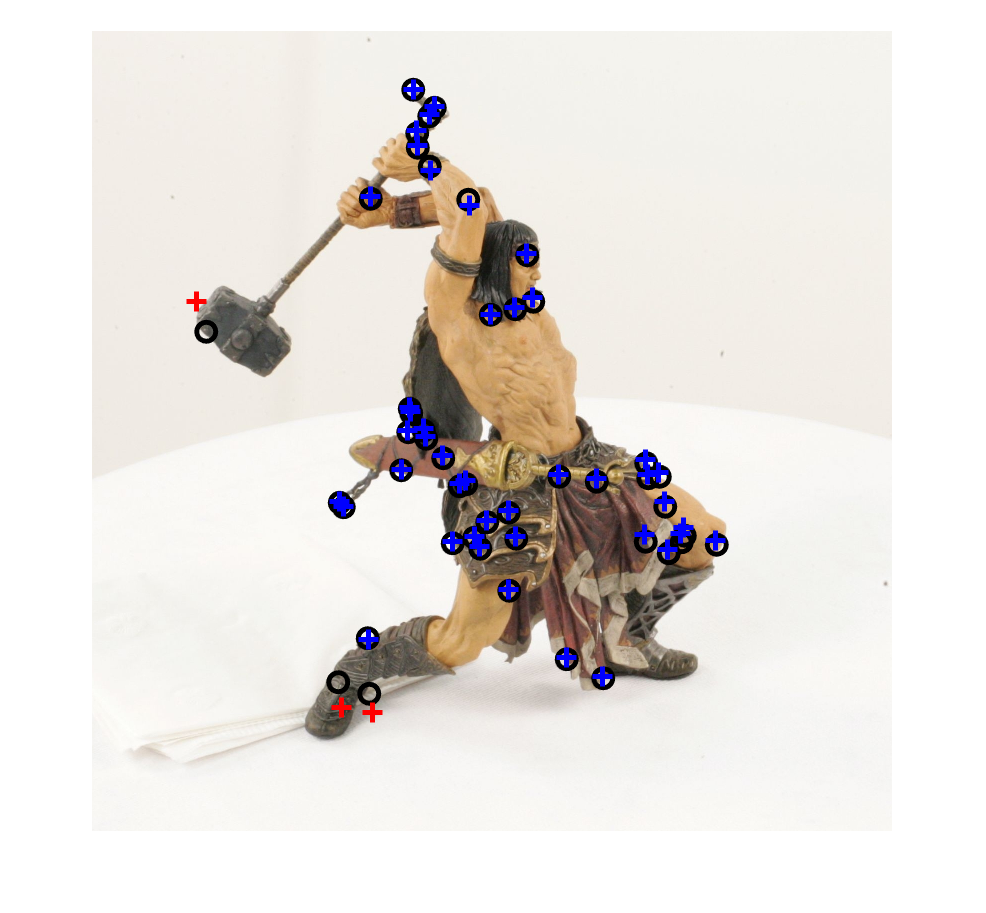
\includegraphics[scale = 0.6]{6_6warrior.png}
\caption{Result of Reprojection: Warrior}
\end{figure}

\newpage
\begin{figure}[!ht]
\centering
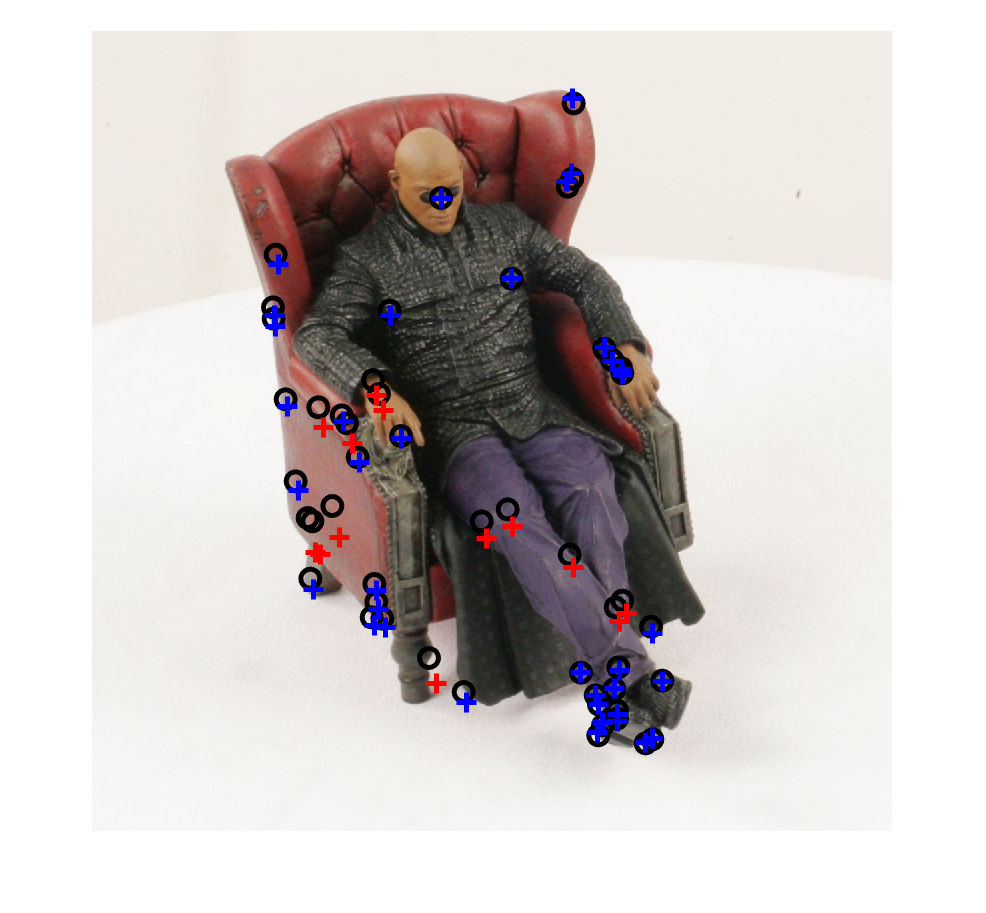
\includegraphics[scale = 0.6]{6_6matrix.png}
\caption{Result of Reprojection: Matrix}
\end{figure} 
 
        

\newpage

\text{\Large{\textbf{Appendix}}}
\lstset{
numbers=left
}

\lstinputlisting[language=MATLAB, caption=Script of Problem 4]{hw2_4.m}

\lstinputlisting[language=MATLAB, caption=loadAndPreprocess.m used in Script of Problem 4]{loadAndPreprocess.m}

\lstinputlisting[language=MATLAB, caption=detectError.m used in Script of Problem 4]{detectError.m}

\lstinputlisting[language=MATLAB, caption=constructHeatMap.m used in Script of Problem 4]{constructHeatMap.m}

\lstinputlisting[language=MATLAB, caption=constructBoundingBox.m used in Script of Problem 4]{constructBoundingBox.m}

\lstinputlisting[language=MATLAB, caption=Script of Problem 5]{hw2_5.m}

\lstinputlisting[language=MATLAB, caption=round2nearest45.m used in Script of Problem 5]{round2nearest45.m}

\lstinputlisting[language=MATLAB, caption=Script of Problem 6]{hw2_6.m}

\lstinputlisting[language=MATLAB, caption=CornerDetect.m used in Script of Problem 6]{CornerDetect.m}

\lstinputlisting[language=MATLAB, caption=SSDmatch.m used in Script of Problem 6]{SSDmatch.m}

\lstinputlisting[language=MATLAB, caption=naiveCorrespondanceMatching.m used in Script of Problem 6]{naiveCorrespondanceMatching.m}

\lstinputlisting[language=MATLAB, caption=correspondanceMatchingLine.m used in Script of Problem 6]{correspondanceMatchingLine.m}

\lstinputlisting[language=MATLAB, caption=Triangulate.m used in Script of Problem 6]{Triangulate.m}

\lstinputlisting[language=MATLAB, caption=findOutliers.m used in Script of Problem 6]{findOutliers.m}

\lstinputlisting[language=MATLAB, caption=interpolateLine.m used in Script of Problem 6]{interpolateLine.m}

\lstinputlisting[language=MATLAB, caption=showMarker1.m used in Script of Problem 6]{showMarker1.m}

\lstinputlisting[language=MATLAB, caption=showMarker3.m used in Script of Problem 6]{showMarker3.m}

\lstinputlisting[language=MATLAB, caption=showMatching.m used in Script of Problem 6]{showMatching.m}

\end{problemlist}
\end{document}
